% Chapter Template

\chapter{Introducción General} % Main chapter title

\label{ChapterIntroGral} % Change X to a consecutive number; for referencing this chapter elsewhere, use \ref{ChapterX}

%----------------------------------------------------------------------------------------
%	SECTION 1
%----------------------------------------------------------------------------------------

\section{Introducción}

FOCUS es un emprendimiento que tiene por objetivo predecir daños en grandes infraestructuras (edificios, minas, represas, etc). Para lograrlo, planifica la construcción de una constelación de satélites que relevarán la posición y movimiento de las instalaciones a monitorear. En caso de detectar grandes desviaciones, disparará una alarma para actuar en consecuencia.

Para realizar el revelamiento de la posición de las instalaciones, cada satélite contará con un radar de apertura sintética (en adelanta SAR, de sus siglas en inglés \textit{synthetic aperture radar}). El sistema SAR consta de 3 etapas bien diferenciadas:
\begin{itemize}
	\item Generación de pulsos, emisión de señales de alta frecuencia (en el caso de este proyecto banda X, que va desde los 8 a 12 GHz) y lectura de rebotes de la señal en la superficie terrestre.   
	\item Procesamiento de las ondas reflejadas del grupo de pulsos para generar una imagen SAR.
	\item Compresión del formato de la imagen para ser enviada mediante la computadora del sistema central a una base terrena.
\end{itemize}

En la figura \ref{fig:diagBloques} se presenta el diagrama en bloques del sistema  con las tres partes principales: sistema radar, procesamiento SAR y computadora del sistema central. El bloque central (recuadro verde en la figura) representa el alcance de las tareas a desarrolladas, que son el procesamiento de señales y la construcción de la imagen SAR.



%-----------------------------------
%	SECTION 2
%-----------------------------------
\section{Objetivo y alcance}

DE LA ESTRUCTURA DE MEMORIA... Sistema Interno del satélite y plataforma en donde se implementó el trabajo

\begin{figure}[htpb]
\centering 
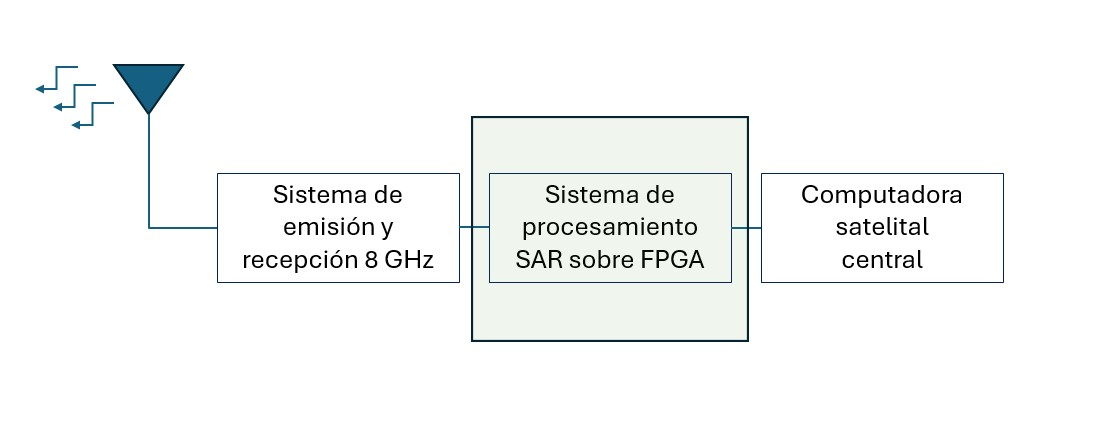
\includegraphics[width=.95\textwidth]{./Figuras/Diagrama Bloque Sistema.jpg}
\caption{Diagrama en bloques del sistema SAR.}
\label{fig:diagBloques}
\end{figure}

\vspace{25px}

%-----------------------------------
%	SECTION 3
%-----------------------------------

\section{Estado del arte}
Morbi rutrum odio eget arcu adipiscing sodales. Aenean et purus a est pulvinar pellentesque. Cras in elit neque, quis varius elit. Phasellus fringilla, nibh eu tempus venenatis, dolor elit posuere quam, quis adipiscing urna leo nec orci. Sed nec nulla auctor odio aliquet consequat. Ut nec nulla in ante ullamcorper aliquam at sed dolor. Phasellus fermentum magna in augue gravida cursus. Cras sed pretium lorem. Pellentesque eget ornare odio. Proin accumsan, massa viverra cursus pharetra, ipsum nisi lobortis velit, a malesuada dolor lorem eu neque.

%----------------------------------------------------------------------------------------
%	SUBSECTION 1
%----------------------------------------------------------------------------------------

\subsection{Sistemas SAR}

Sed ullamcorper quam eu nisl interdum at interdum enim egestas. Aliquam placerat justo sed lectus lobortis ut porta nisl porttitor. Vestibulum mi dolor, lacinia molestie gravida at, tempus vitae ligula. Donec eget quam sapien, in viverra eros. Donec pellentesque justo a massa fringilla non vestibulum metus vestibulum. Vestibulum in orci quis felis tempor lacinia. Vivamus ornare ultrices facilisis. Ut hendrerit volutpat vulputate. Morbi condimentum venenatis augue, id porta ipsum vulputate in. Curabitur luctus tempus justo. Vestibulum risus lectus, adipiscing nec condimentum quis, condimentum nec nisl. Aliquam dictum sagittis velit sed iaculis. Morbi tristique augue sit amet nulla pulvinar id facilisis ligula mollis. Nam elit libero, tincidunt ut aliquam at, molestie in quam. Aenean rhoncus vehicula hendrerit.

%----------------------------------------------------------------------------------------
%	SUBSECTION 2
%----------------------------------------------------------------------------------------

\subsection{Algoritmos}

Sed ullamcorper quam eu nisl interdum at interdum enim egestas. Aliquam placerat justo sed lectus lobortis ut porta nisl porttitor. Vestibulum mi dolor, lacinia molestie gravida at, tempus vitae ligula. Donec eget quam sapien, in viverra eros. Donec pellentesque justo a massa fringilla non vestibulum metus vestibulum. Vestibulum in orci quis felis tempor lacinia. Vivamus ornare ultrices facilisis. Ut hendrerit volutpat vulputate. Morbi condimentum venenatis augue, id porta ipsum vulputate in. Curabitur luctus tempus justo. Vestibulum risus lectus, adipiscing nec condimentum quis, condimentum nec nisl. Aliquam dictum sagittis velit sed iaculis. Morbi tristique augue sit amet nulla pulvinar id facilisis ligula mollis. Nam elit libero, tincidunt ut aliquam at, molestie in quam. Aenean rhoncus vehicula hendrerit.
